\documentclass[11pt]{beamer}
\usetheme{Warsaw}

\definecolor{mygreen}{rgb}{.125,.5,.25}
\usecolortheme[named=mygreen]{structure}



% Packages
\usepackage[utf8]{inputenc}
\usepackage[english]{babel}
\usepackage{amsmath}
\usepackage{amsfonts}
\usepackage{amssymb}
\author{Jaskeerat Singh Saluja(2019MT60752)}
\title{ELL-409 Assignment}
%\setbeamercovered{transparent} 
%\setbeamertemplate{navigation symbols}{} 
%\logo{} 
%\institute{} 
%\date{} 
%\subject{} 
\begin{document}

\begin{frame}
\titlepage
\end{frame}



%\begin{frame}{Title of the frame}
%\tableofcontents
%\end{frame}


\begin{frame}{Intro}
\begin{huge}
Pre-requisites
\end{huge} 
\end{frame}


%Prereq
\begin{frame}
\textbf{Normalizing Data}

While generating the design matrix we  normalize the features vectors i.e $x,x^2,x^3....x^M$ .
The feature X $\in$ [-M,M] , then the features $X^2 \in$ $[-M^2,M^2]$ , and so on for all other powers of X. 
Hence the loss function (least squared error) forms contours with elliptical shapes . 

Hence while optimizing error in the gradient descent algorithm , an improvement in $X^2$ may cause big step in $X$, thus instead of decreasing error ,we may cross the minima point , and error may increase . This would cause a lot of oscillation of $w$ around the minima point.

\textbf{An unnormalized data would causes:}
\begin{itemize}
\item highly sensitive learning parameter
\item high oscillation of parameter $w$ during convergence

\end{itemize}


To prevent this we use normalization techniques like z-normal and min-max normalization. This transforms the contour plots of loss function to circular shapes , hence the gradient descent converges better
\end{frame}

\begin{frame}
\textbf{Z-Normalization:} The feature vector is transformed as  $$(X) -> \frac{X-\mu}{\sigma}$$
where $\mu :$ mean of the feature vector and $\sigma$ : variance of the feature.

\textbf{Z-Normalizing feature vector :} {$x,x^2,... x^M$}is transformed as  $$x^i -> \frac{(x^i-mean(x^i)}{\sigma(x^i}$$.

Running gradient descent yield us $w_0^* ,w_1^* ... w_M^*$ . Which optimizes error for our normalized data points X. Thus we need to 'un-normalize' the parameters $W$ to previous space

The \textbf{unnormalized parameter} we get are $$w_i = \frac{w_i^*}{\sigma_i} , \forall i \in \{1,M\} and $$
$$w_0 = w_0^* - \sum_{i=1}^{i=M} {\frac{\mu_i}{\sigma_i}}$$
\end{frame}

\begin{frame}
\textbf{The code written for polyfit auto-normalizes the feature space before training and unnormalize the paramter w after training.}

Normalization class is also implemented which is inherited by polyfit class.
\end{frame}


%% Part-1A
\begin{frame}
\begin{huge}
Part-1A
\end{huge}
\end{frame}
\begin{frame}{1A - (a) Fitting First 20 points}
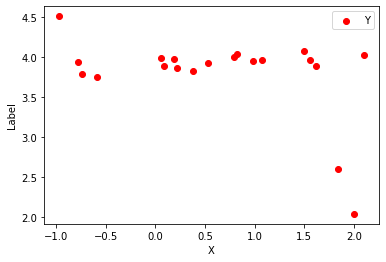
\includegraphics[scale=0.5]{images/plot20points.png} 
\end{frame}


\begin{frame}{1A - (a) Fitting First 20 points}
\textbf{Polyfit using Gradient Descent}
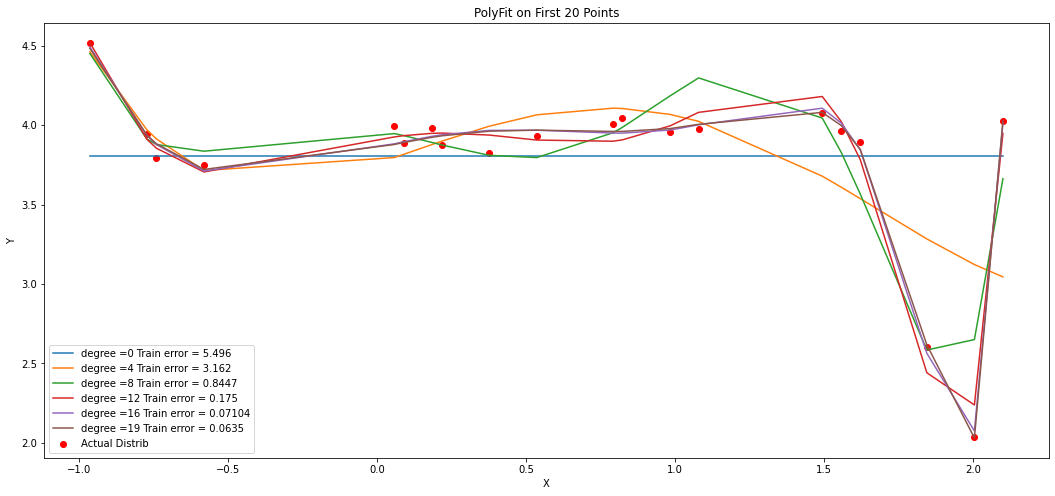
\includegraphics[scale=0.3]{images/polyfitgradientdescent.png}
\end{frame}

\begin{frame}{1A - (a) Fitting First 20 points}
\textbf{Polyfit using Gradient Descent}
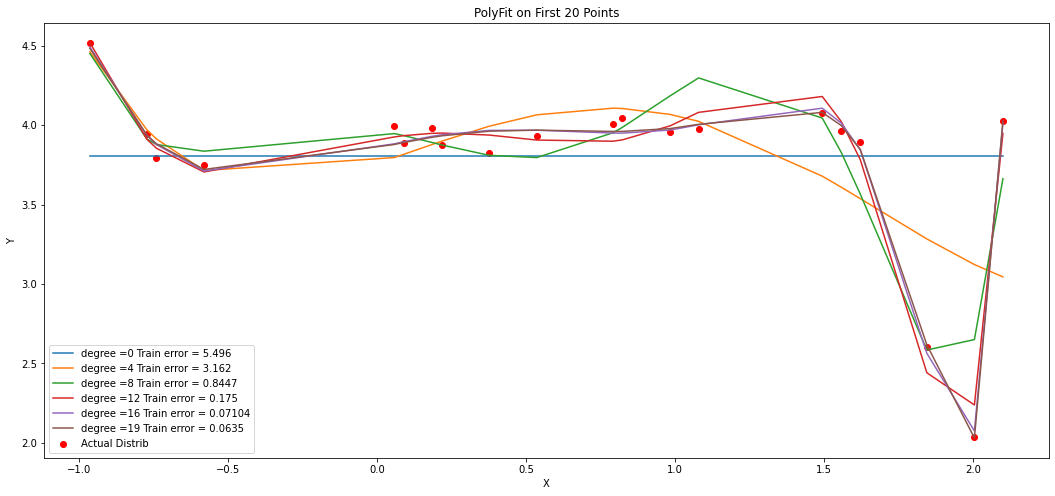
\includegraphics[scale=0.3]{images/polyfitgradientdescent.png}
\end{frame}

\begin{frame}
\textbf{Training error vs Degree of Polynomial}
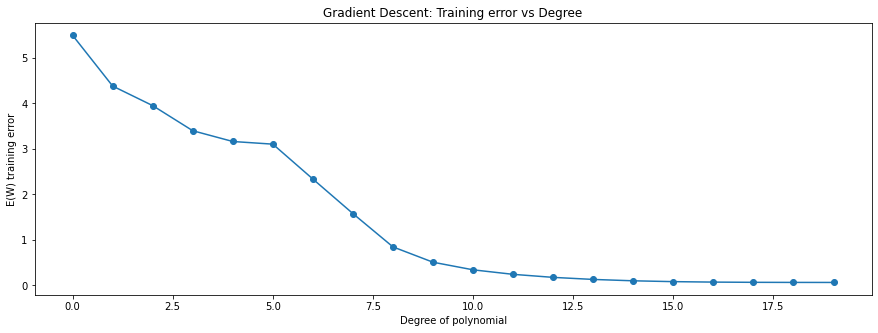
\includegraphics[scale=0.3]{images/3.png}
\end{frame}
\textbf{Training error vs Number of Iterations}
From below we can say the gradient descent algorithm converges very fast for the first 5000 iteration , after that the convergence of gradient descent is very slow in successive iteration. Here 1 iteration corresponds to 1 pass over the data set , hence in our case 1 iteration implies 1 pass over all 20 points.


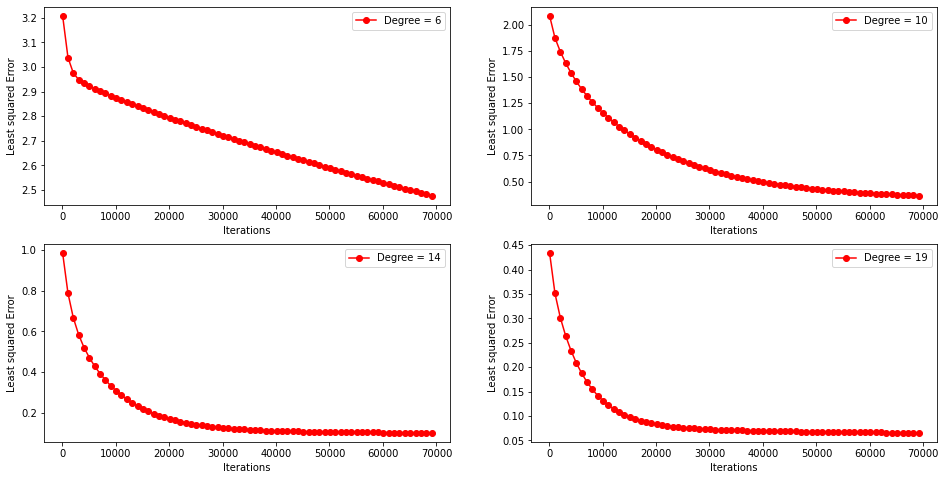
\includegraphics[scale=0.25]{images/4.png}
\begin{frame}
\textbf{Variation of Error} $E(W)$ \textbf{with the batch size in gradient descent¶}\\
Since the data set is quite small i.e only 20 points . Also the data was normalized before the grad desccent thus the batch gradient descent performed similar on all batches.

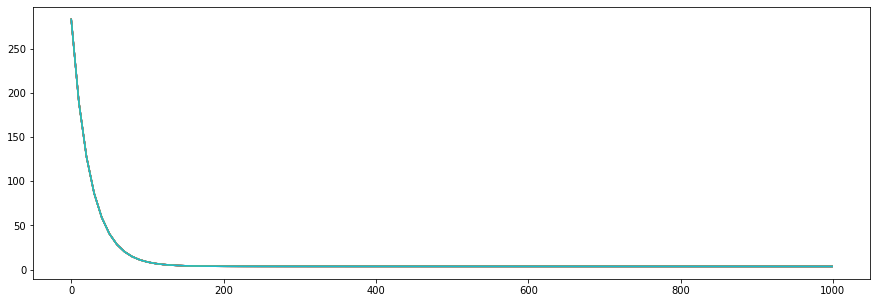
\includegraphics[scale=0.5]{images/5.png}
\end{frame}

\begin{frame}
\textbf{\large{Optimization using psedo penrose Inverse}}
\end{frame}


\begin{frame}
\textbf{Polyfit using PIV}
Observations: Starting  $degree > 16$  the PIV fails , thus gives poor fitting , as shown below.This is the reason we cannot rely on PIV method for fitting higher degree poynomials on our data set
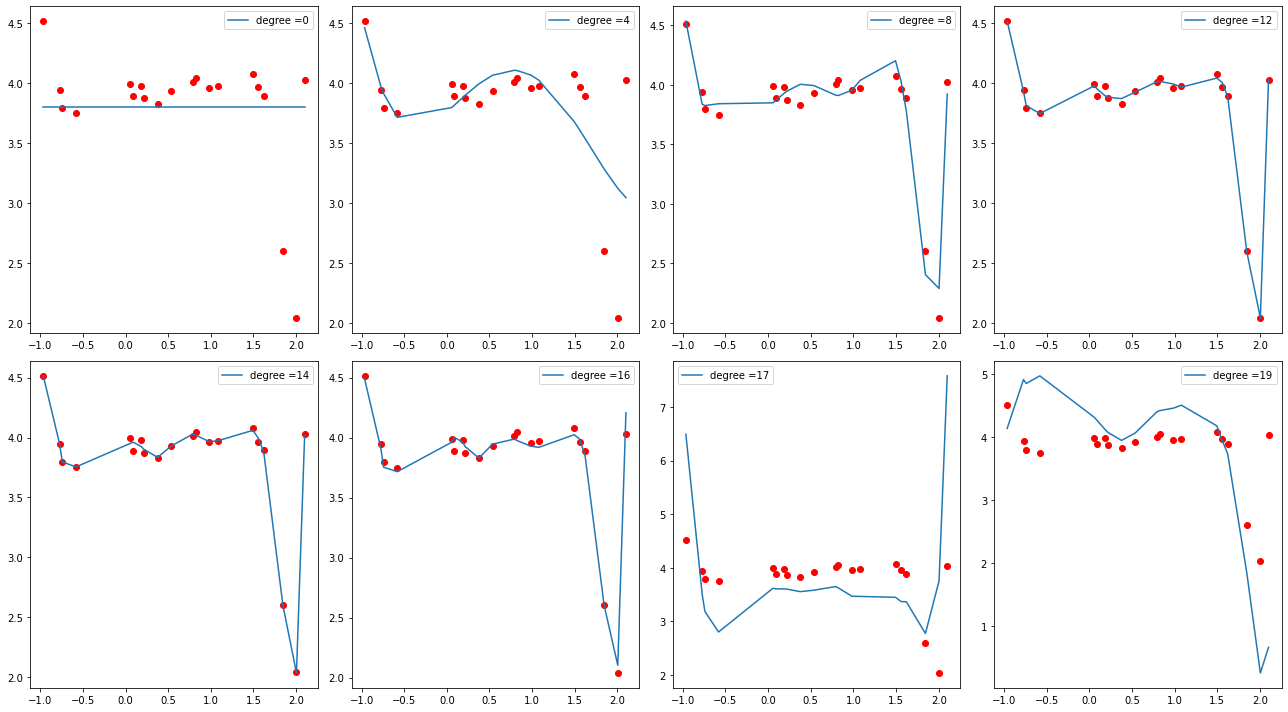
\includegraphics[scale=0.25]{images/6..png}
\end{frame}

\begin{frame}
\textbf{Error vs degree of poynomial }\\
Since PIV fails for $degree \geq 15$ hence the error shoots up
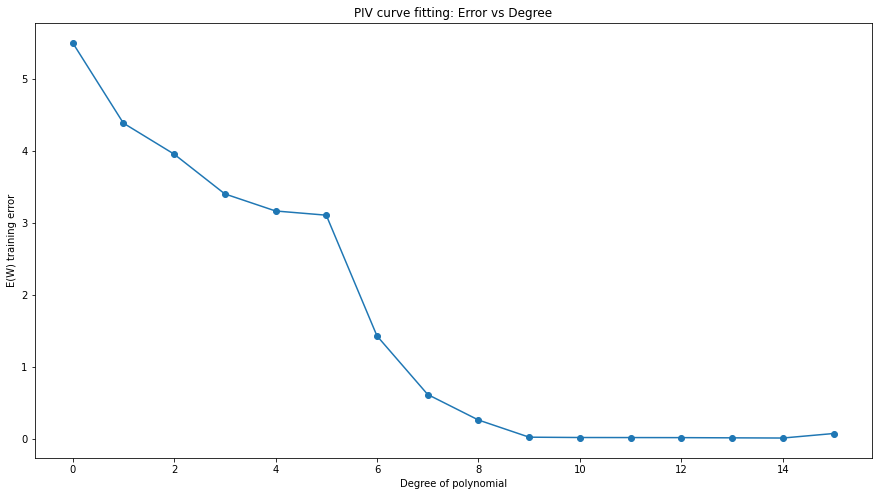
\includegraphics[scale=0.3]{images/7.png}
\end{frame}

\begin{frame}
\textbf{Good fit of polynomial (Underfitting , overfitting) (without regularization)}\\
We know the  $\textbf{train error} -> 0$ as the degree of poynomial M increases but this lead to overfitting of the model over the underlying data set.

Test validation 
To test a model we will partition our data i.e 20 points into test and train data . The model is trained on trained data and scored on the test data. 

Several models are scored using above schema , one with the best score i.e in our case the least error is chosen.

\textbf{I have used K-fold cross validation method to score the models with variable hyper-paramters}

The k-fold cross validation method is implemented in file cross-validation.py
\end{frame}



\begin{frame}
\textbf{K-Fold Cross Validation On our data set. }
Observation: The polynomial of $degree=9$ is sweet spot . Thus $degree=9$ gives us a good fit .\\
$w_{ML}$ =[ 3.99399065 ,-0.56158887, -0.16833793 , 4.93082264, -2.41734063 ,-8.69985778,
  6.99587172  ,3.09004417 ,-4.22105658 , 1.00545962]
  \\
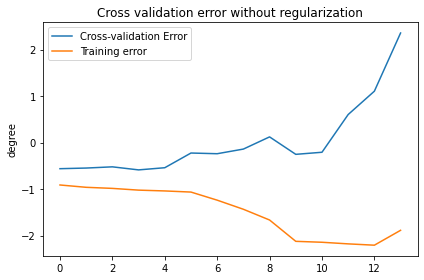
\includegraphics[scale=0.40]{images/9.png}
\end{frame}

\begin{frame}
Estimation of noise 
$$\frac{1}{\beta_{ML}}= \frac{\sum{(y-t)^2}}{N}$$.
Since our best approximation comes for degree 9 . Thus $variance =\frac{1}{\beta}$. Hence Gaussian distribution$N((\mu= 0,\sigma=0.03558) $describes the underlying noise.

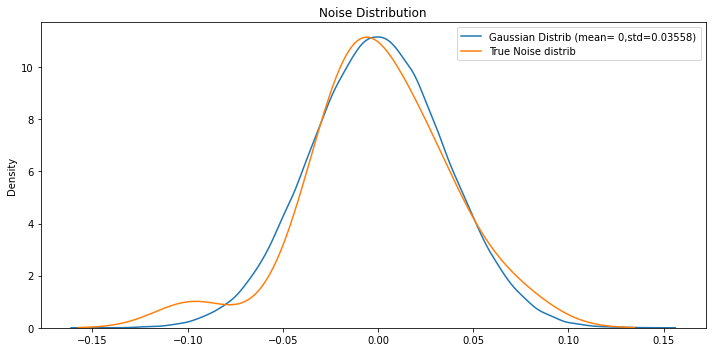
\includegraphics[scale=0.5]{images/27.png}
\end{frame}


\begin{frame}
Observations:
\begin{itemize}

\item The points 20 are too low in number thus we donot get the an expected $U$ shaped curved depicting decrese in $(bias)^2$ and increase in $variance$ ,giving an sweet-spot in between.
\item The error is contributed from following:
\begin{itemize}[]
    \item test variance (= variance due to test sample size) : Since the test points are too low in our model thus the test error itsef have a high variance.
    \item Model instability variance due to training sample size
    \item testing bias
\end{itemize}
	\item We know that  at lower degree of polynomial the cross validation should be dominated by bias in model ,but due to so low count of data points the bias does-not dominate that well over the data , hence the variance starts dominating soon.

\item At $degree =9$ there is  dip in the CVR , hence we get a see spot where the total bias and variance sum is minimized. 
For $degree\geq 10$ , the variance starts shooting up
\end{itemize}

\end{frame}



\begin{frame}
\textbf{Bayesian curve fitting} .


Interested values of $\lambda = [10^{-1.0},10^{-1.2},10^{-1.4},...10^{-4.8}]$
Interested values of $degree=$ [9,10,11,12,13,14]

\textbf{Approach}: Iterate over all (lambda ,degree) pairs , calculate the cross validation test error. One with least test error as good fit for our .
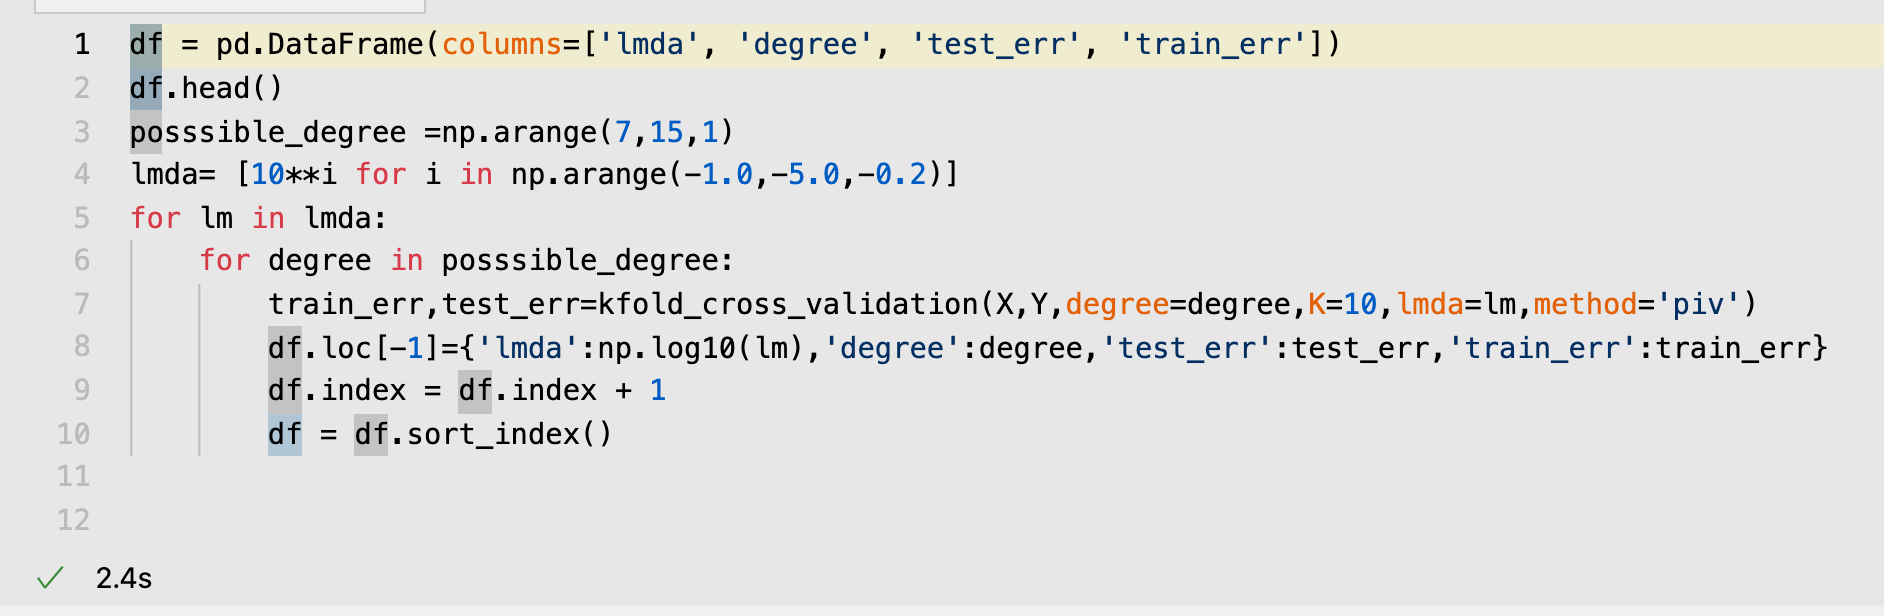
\includegraphics[scale=0.35]{images/29.png}

\end{frame}





\begin{frame}
\textbf{Tuning of the hyper-parameter continued}
sorting the data Frame by train error gives us that $lmda=10^{-4.2}$and $degree=11$ fits our model with least test error.Hence we found sweet spot of our model using regularization.
\\
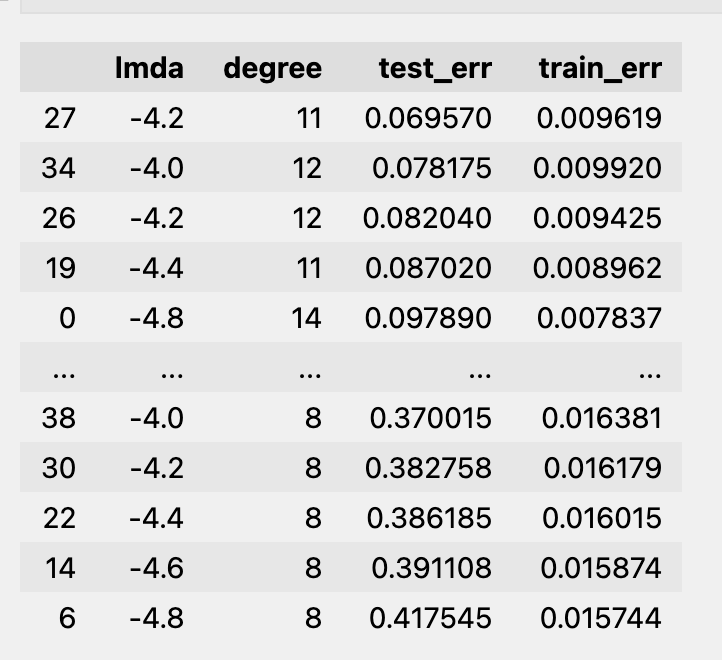
\includegraphics[scale=0.35]{images/38.png}


\end{frame}


\begin{frame}
Estimation of noise (we derived that $\beta$ parameter for both bayesian and maximum likelihood approach gives us same noise distribution, i.e
$$\frac{1}{\beta_{MAP}}= \frac{\sum{(y(x,w)-t)^2}}{N}$$.

Since our best approximation comes for degree 11 and $\lambda=10^{-4.2}$ . Thus $variance =\frac{1}{\beta_{MAP}}$. Hence Gaussian distribution$N(\mu= 0,\sigma=0.0460762419) $describes the underlying noise.
$w_{MAP}$=[ 4.00508911e+00 -2.32331032e-02 -7.08705280e-01  1.34058586e+00
 , 1.09848573e+00, -3.16688496e+00 , ,4.49931451e-01  ,1.58108297e+00
 ,-5.82997950e-01 , 6.70898630e-02 ,-1.18962016e-01  ,1.58515472e-02
 , 2.62794355e-03 , 7.11685818e-03 ,-1.34651068e-03]\\

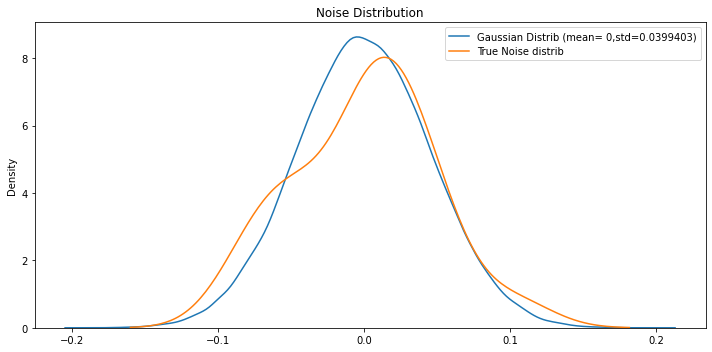
\includegraphics[scale=0.2]{images/31.png}
\end{frame}


%100 points data set
\begin{frame}
\textbf{Using Full 100 points dataset}
\end{frame}

\begin{frame}
\textbf{Polynomial fit over our dataset}\\ 
Optimization using Gradient descent
Even after  \textbf{20,000 iteration iterations per model} (took minutes to just train)  , gradient descent could not optimize the polynomial fit , very well. 
I have used moment based gradient descent which is faster than batch gradient descent , but  not fast enough to converge at a faster rate.

In the next slide we see that better fit by pseudo penrose inverse formulation

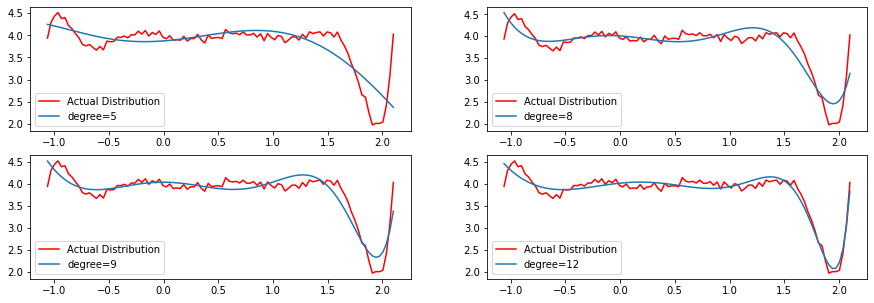
\includegraphics[scale=0.28]{images/34.png}


\end{frame}


\begin{frame}
\textbf{Least squared  error vs degree}
Clearly $degree \geq 9 $ we get a good fit over our dataset.

Still , the convergence of gradient descent is quite slow, need high speed computers to train. But gradient descent converges to minima and does not have issue when design matrix is singular
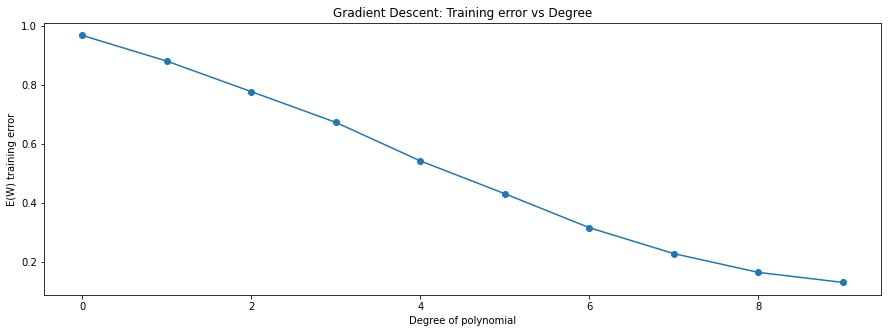
\includegraphics[scale=0.27]{images/35.png}
\end{frame}

\begin{frame}
\textbf{Errors vs number of iterations} in gradient descent. The below picture clearly depicts the rate at which gradient descent converges.
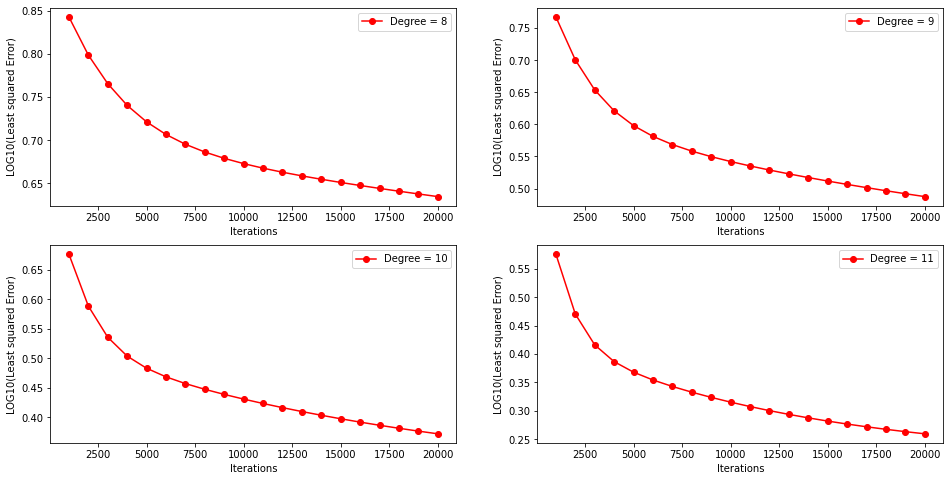
\includegraphics[scale=0.3]{images/36.png}
\end{frame}


\begin{frame}
\textbf{Polynomial fit over our dataset} 
Optimization using PIV (pen-rose inverse matrix)


\textbf{$Degree=9$(least complexity) polynomial fits our curve nicely.}
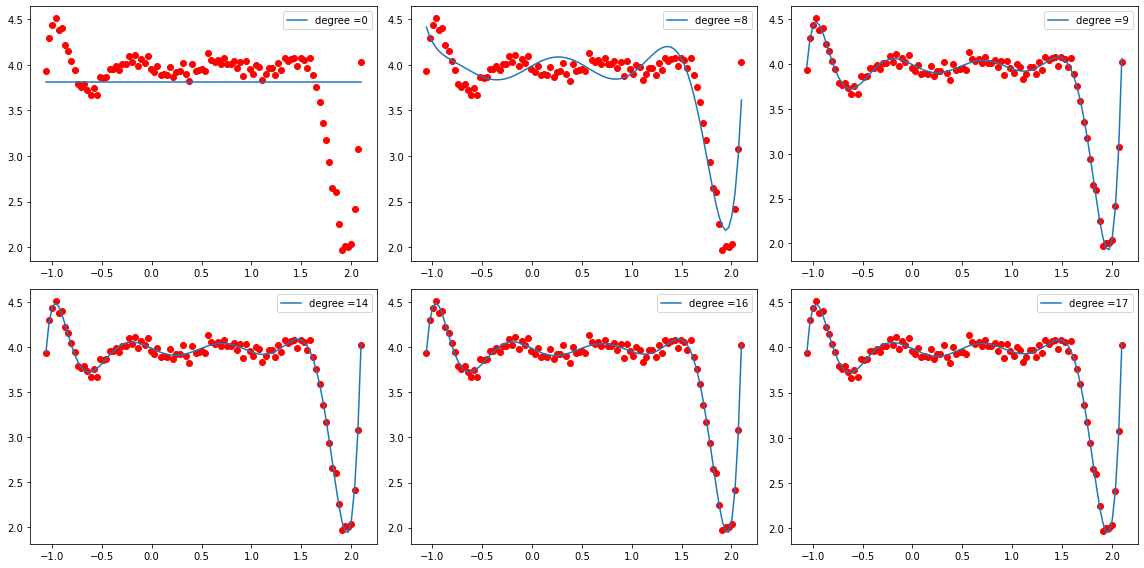
\includegraphics[scale=0.28]{images/14.png}


\end{frame}



\begin{frame}
\textbf{Training error vs degree}
Clearly $degree \geq 9 $ we get a good fit over our dataset
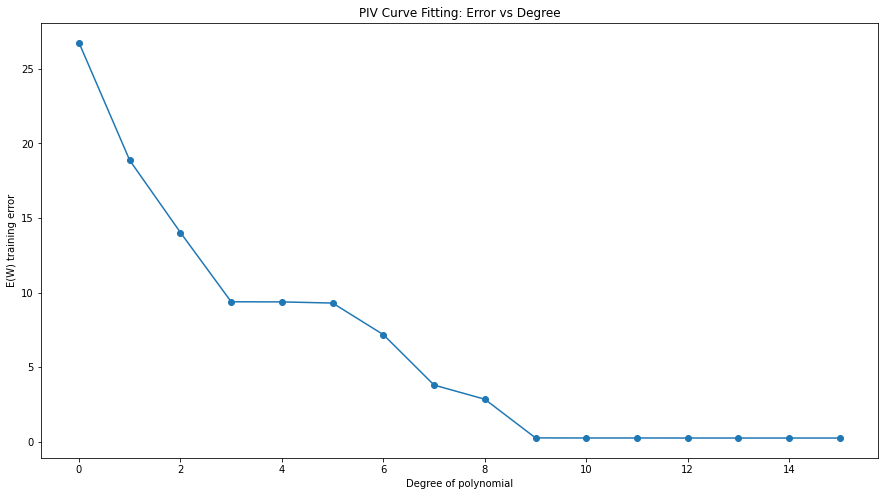
\includegraphics[scale=0.27]{images/15.png}
\end{frame}


\begin{frame}
\textbf{Maximum Likelihood }\\
I have used K-fold cross validation method to score the models with variable hyper-paramters
paramter 

Clearly $M=9$ is polynomial with least complexity that gives us the sweet spot over our data set.

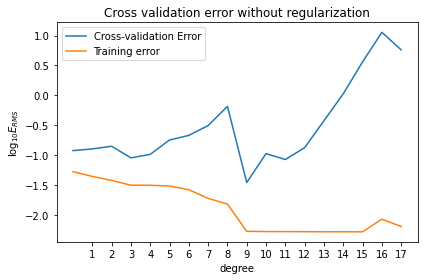
\includegraphics[scale=0.50]{images/16.png}
\end{frame}

\begin{frame}
\begin{Huge}
Observations:
\end{Huge}
\begin{itemize}
\item The points 100 are good in number thus we have smoother training and test error over our data set. 
\item Due to enough points the cross validation error is smooth as function of degree of the polynomial. 
\item $degree=9$ is the lowest degree which fits our data set nicely.
\item Hence polynomial of $degree =9$ fits our data well (low train and test error)

\item region ($degree<9$ high training error $->$ Under-fitting)
\item region ($degree \geq 10 $ high testing error $->$ over fitting)
\end{itemize}
\end{frame}

\begin{frame}

Estimation of noise 
$$\frac{1}{\beta_{ML}}= \frac{\sum{(y-t)^2}}{N}$$.
Since our best approximation comes for degree 9 . Thus $variance =\frac{1}{\beta}$. Hence Gaussian distribution$N((\mu= 0,\sigma=0.0511478) $describes the underlying noise.

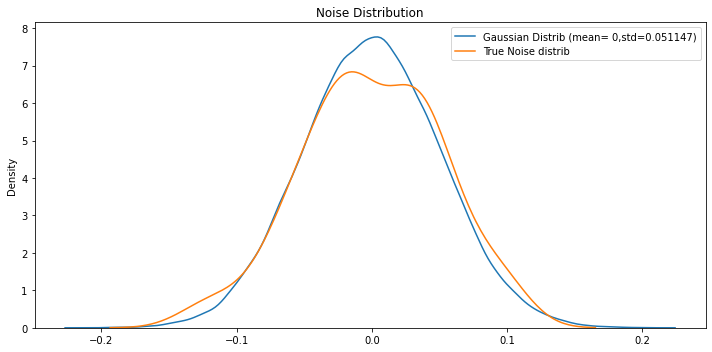
\includegraphics[scale=0.35]{images/28.png}
\end{frame}

% Regularizatin on 100 points

\begin{frame}
Bayesian curve fitting .


Interested values of $\lambda = [10^{-1},10^{-2},10^{-3},10^{-4}...10^{-20}]$
Interested values of $degree=$ [9,10,11,12,13,14]

Approach: Iterate over all (lambda ,degree) pairs , calculate the cross validation test error. One with least test error as good fit for our .
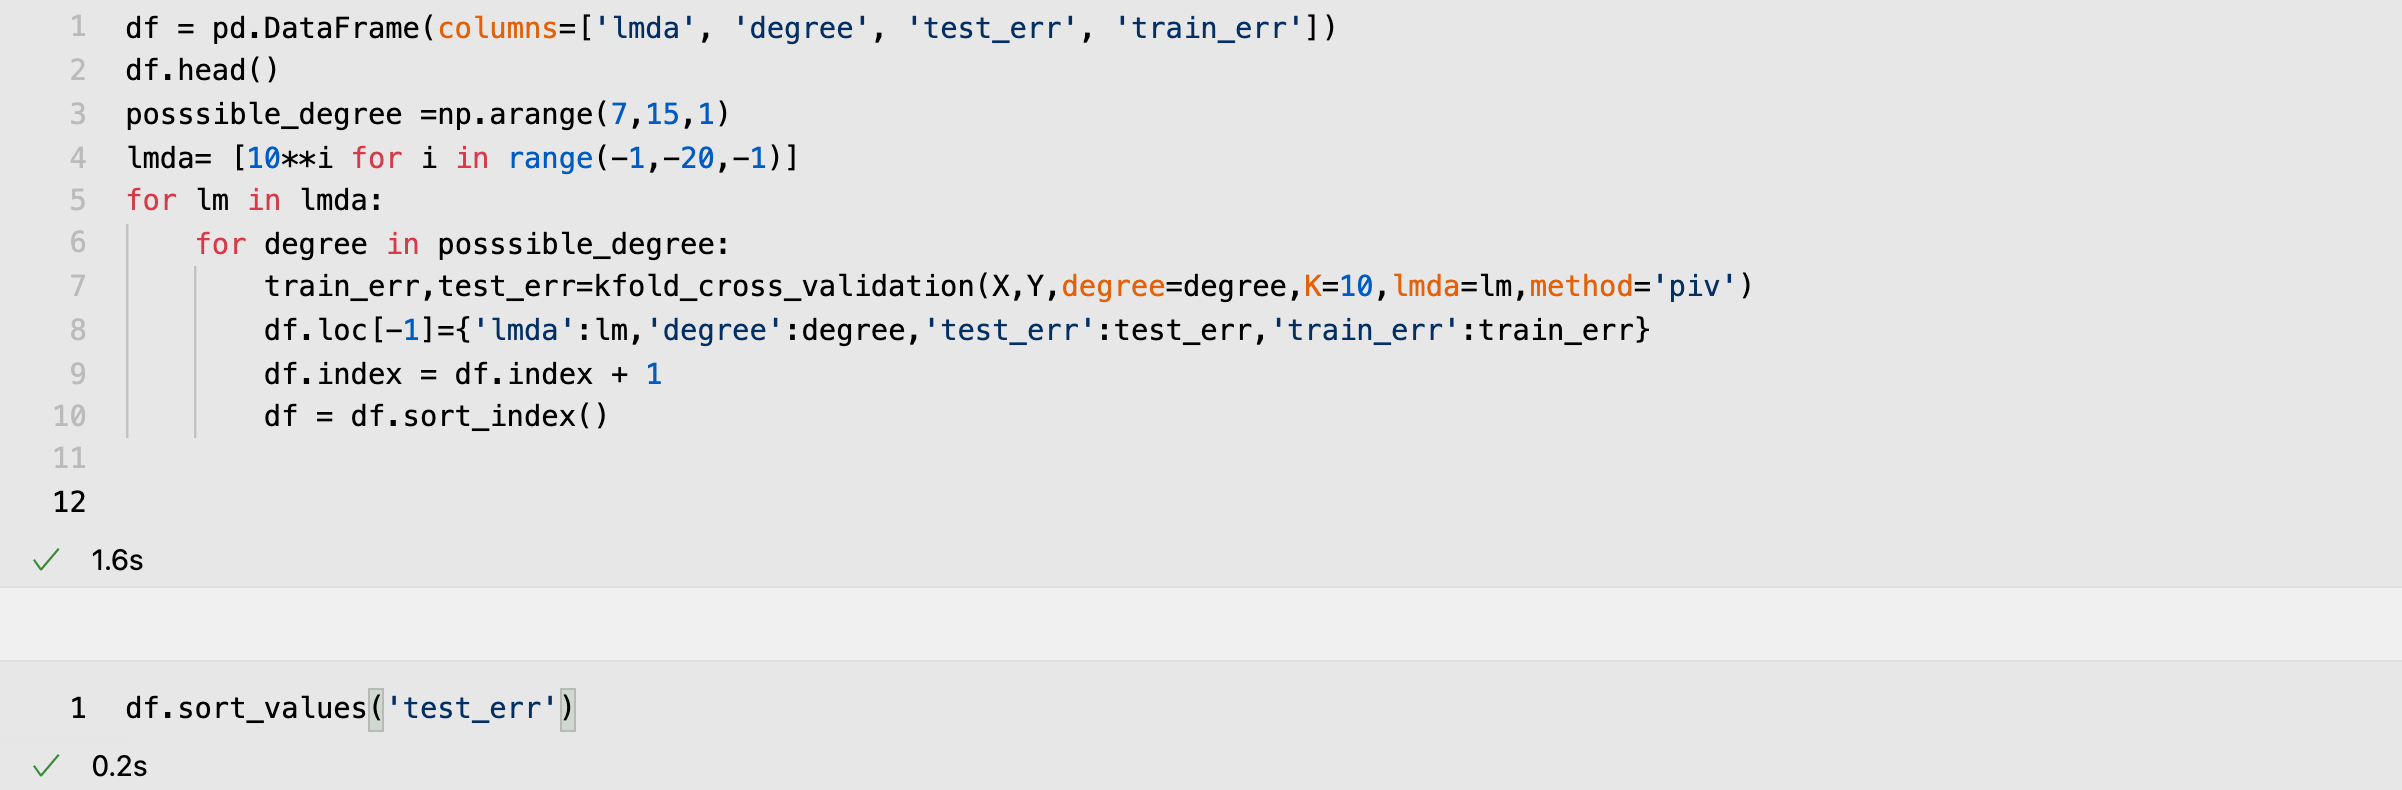
\includegraphics[scale=0.35]{images/11.png}

\end{frame}





\begin{frame}
\textbf{Tuning of the hyper-parameter continued}
sorting the data Frame by train error gives us that $lmda=10^{-17}$and $degree=9$ fits our model with least test error.Hence we found sweet spot of our model using regularization.
\\
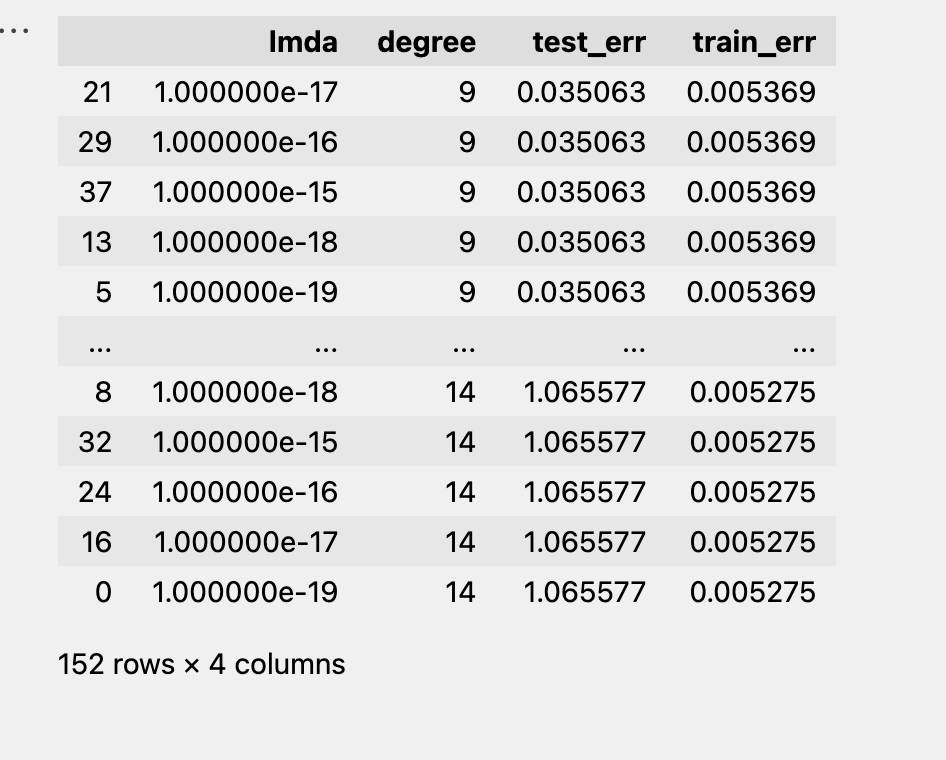
\includegraphics[scale=0.27]{images/12.png}


\end{frame}

\begin{frame}

Estimation of noise 
$$\frac{1}{\beta_{MAP}}= \frac{\sum{(y-t)^2}}{N}$$.
Since our best approximation comes for degree 9 and $\lambda=10^{-17}$. Thus $variance =\frac{1}{\beta}$. Hence Gaussian distribution$N((\mu= 0,\sigma=0.0511478958) $describes the underlying noise.

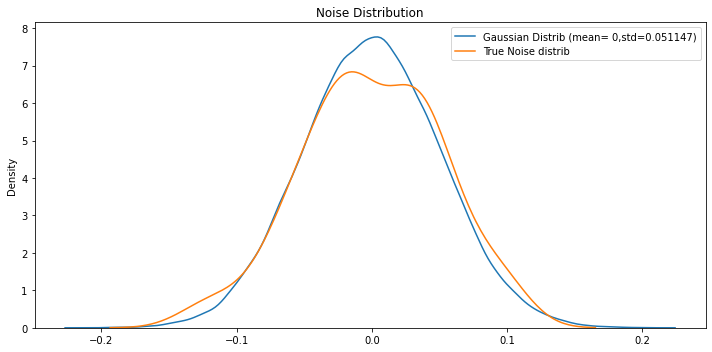
\includegraphics[scale=0.35]{images/28.png}
\end{frame}


\begin{frame}
Final estimate of polynomial is poynomial with degree=9 and regularization $\lambda=10^{-17}$. Since it is one with minimum cross validation error. Also it prevents over fitting by penalizing higher values.

The parameters w is $[w_0=3.99399065,w_1= -0.56158887, -0.16833793, $ $4.93082264, -2.41734063 ,-8.69985778,6.99587172$  $,3.09004417 ,-4.22105658 , w_9=1.00545962]$
\end{frame}






%%Part 1-B
\begin{frame}

\begin{Huge}
Part-1B
\end{Huge}
\end{frame}



\begin{frame}
\textbf{Polynomial Fit over the given points}.
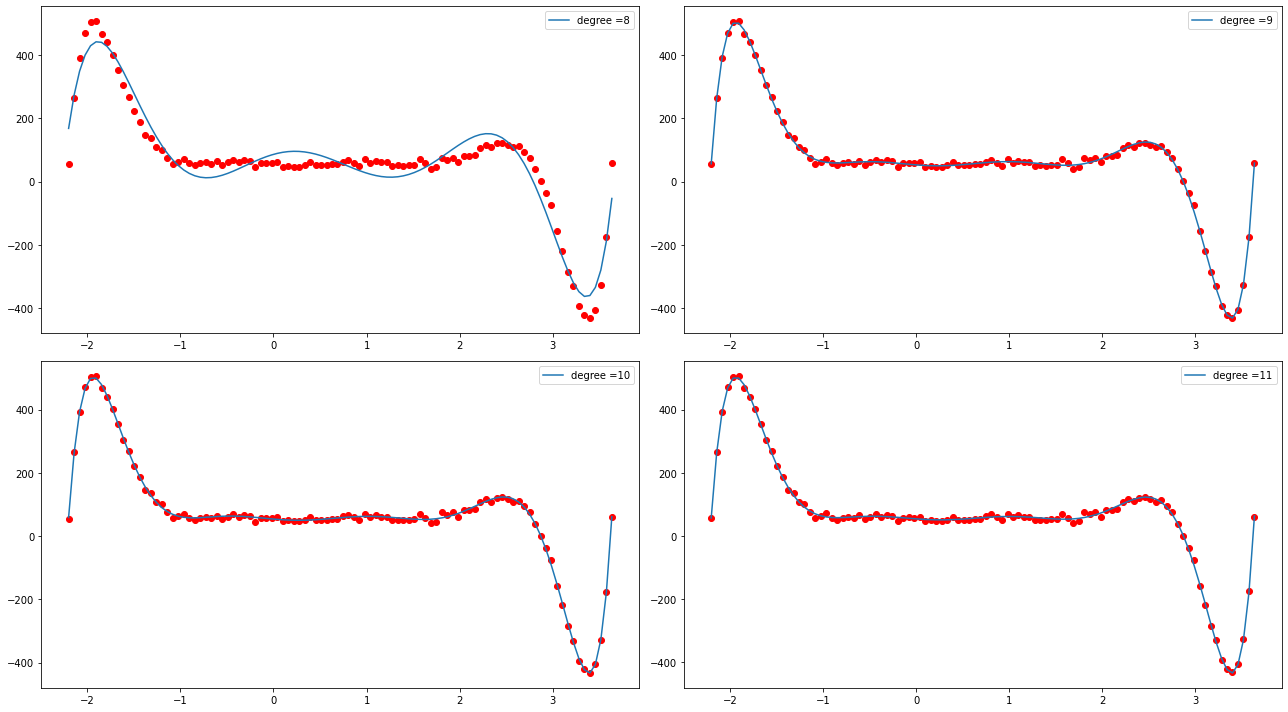
\includegraphics[scale=0.25]{images/19.png}
\end{frame}


\begin{frame}
\textbf{Maximum Likelihood Approach}
The below plots indicated that $degree=9$ is the best fit for our model as it attains low training error and test error(cross validation).
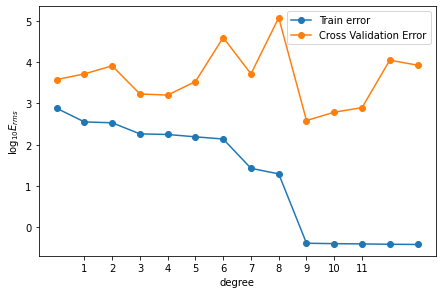
\includegraphics[scale=0.5]{images/21.png}
\end{frame}



\begin{frame}
\textbf{Bayesian Curve Fitting}\\
Regularizing on various values of $\lambda$. 
Interested values are $\lambda=[10,1,10^{-1},10^{-2},10^{-3}...10^{-15}]$ and  $degree=[9,10,11,12,13]$.
The below approach trains over all combinations of $\lambda$ and $degree$. 
The combination with least test error(validation) is chosen.
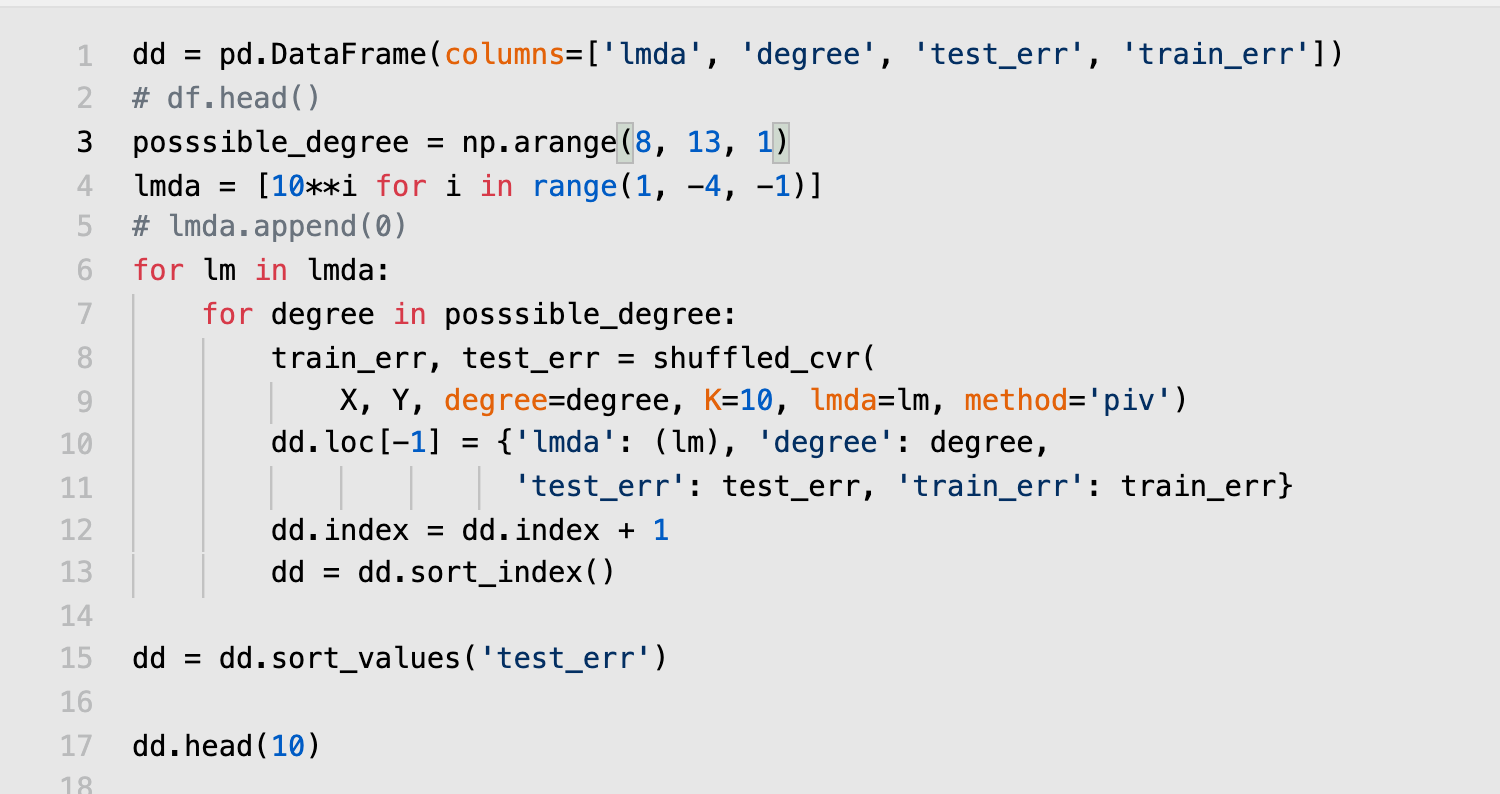
\includegraphics[scale=0.40]{images/22.png}
\end{frame}

\begin{frame}
\textbf{Bayesian Curve Fitting}\\
Sorting the dataframe on basis of the "training error" , we get a good regularization for $degree=9$ and $\lambda=10^{-7}$. \textbf{Choosing low degree and high regularization when similar results over all combinations.}
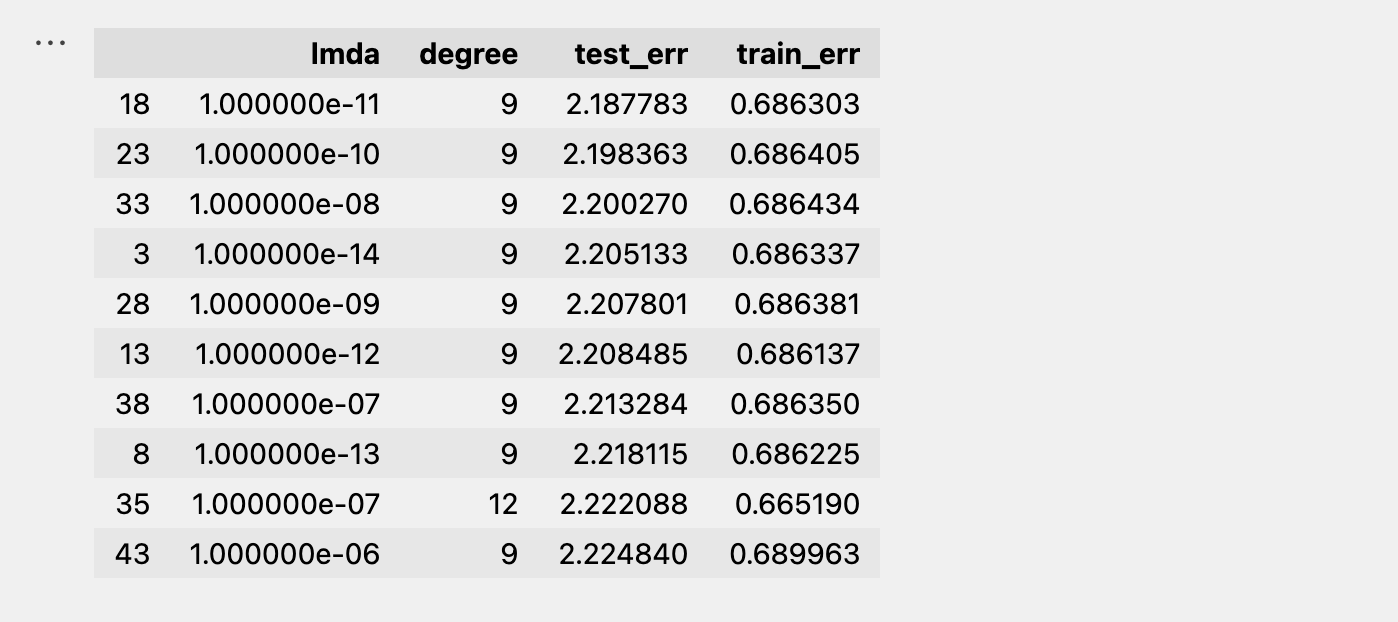
\includegraphics[scale=0.5]{images/32.png}
\end{frame}




\begin{frame}
Noise: Since the true data has inherent noise in it's data , the below plot helps visualizing noise.
Even if we fit the below data with high degree, we may end up fitting the noise , thus leads to over fitting.
$noise = h(x) -t$
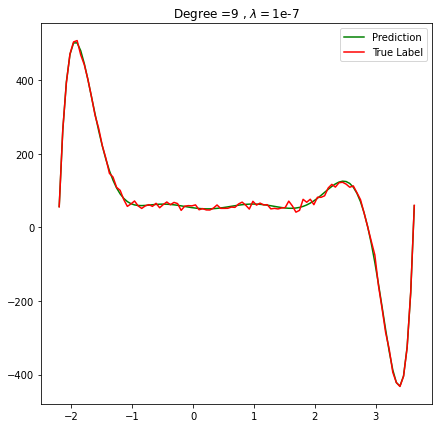
\includegraphics[scale=0.4]{images/24.png}
\end{frame}

\begin{frame}
The noise in underlying distribution has a mean of $-6.65686718797076 *10^{-7}$, which is quite close to 0. Also noise lies in interval $[-20,20]$. We can test if the underlying noise is beta distribution.

Since beta distribution $ (\alpha,\beta)$ lie in $[0,1]$ with mean of $\frac{\alpha}{\alpha+\beta}$. 

We scale our noise distribution to lie in interval [-0.5,0.5] by dividing whole by noise values by 40.
Since mean of our  $noise_{normalized}$ distribution is close to 0 .The shifted noise distribution by factor of 0.5 would lies in [0,1] ,which gives a mean close to 0.5.

We can assume mean of $noise_{normalized}$ to be 0.5 . Comparing it with beta distribution gives us 
$$\frac{\alpha}{\alpha+\beta}=\frac{1}{2}$$
$$\alpha=\beta$$


\end{frame}


\begin{frame}
Thus we plot various $\beta(\alpha,\alpha)$ distribution in comparison to our normalized noise distribution , to get best estimate for our normalized noise. 

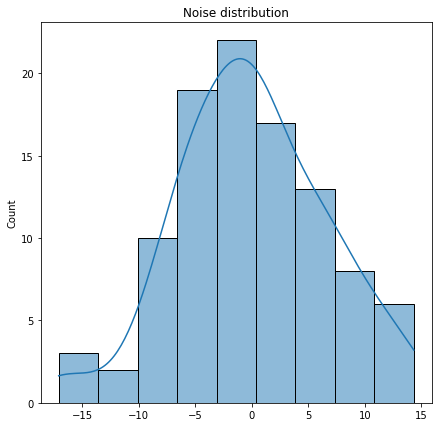
\includegraphics[scale=0.4]{images/25.png}
\end{frame}
\begin{frame}
below comparative plot gives us good estimation of our normalized distribution . Since by inspection $\alpha=4.5$ gives us good estimation. Thus we have
$$noise_{normalized}=\beta(4.5,4.5)$$
$$noise=40 * \beta(4.5,4.5)$$
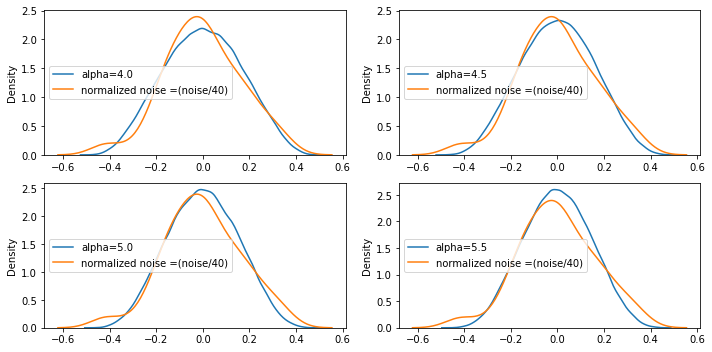
\includegraphics[scale=0.4]{images/26.png}
\end{frame}










%Part-2
\begin{frame}
\begin{Huge}
Part-2 (estimating time series )
\end{Huge}
\end{frame}

\begin{frame}
Visualizing the trends and seasonality of the series.
The box plot tells that there is not much variation of the series over the years, but is periodic every 12 months.
Observation : The range of values in a month is of length at max 5 .
Thus we can model each month separately assuming Gaussian distribution of hypothesis error. 

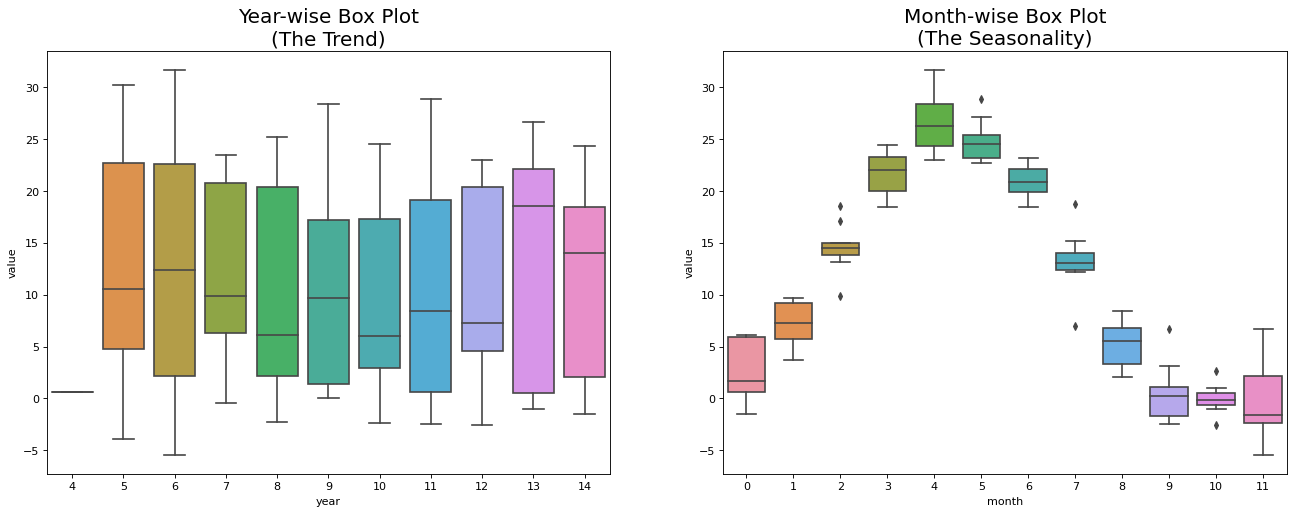
\includegraphics[scale=0.25]{images/33.png}

\end{frame}

\begin{frame}
Since periodic ,the prediction of value would be linear combination of given month's value.  We train a model for each month , by fitting a polynomial over the  index value of  dates with same month.

$$indexval_{date} = (month -1)+(year-2000)*12 $$
for example 1 jan 2020 , we will have $0+20*12 =240$ as its index value.

\textbf{Training}
Using above index value for each date is calculated . 
Then we train the dates with  same months with input as their index value and output as the label. Polyfit is implemeted on these models.

\textbf{Predictions}\\
Depending on the month , the value is predicted on date's month
\end{frame}

\begin{frame}
The models were trained using regularization , coupled with cross-validation. Copying all images for all 12 models to this presentation would be an overkill , thus I haven't included them in the presentation. Although there is Jupyter notebook with name \textbf{P2.ipynb} , where the models trained are represented. 
The final hyper paramter used were
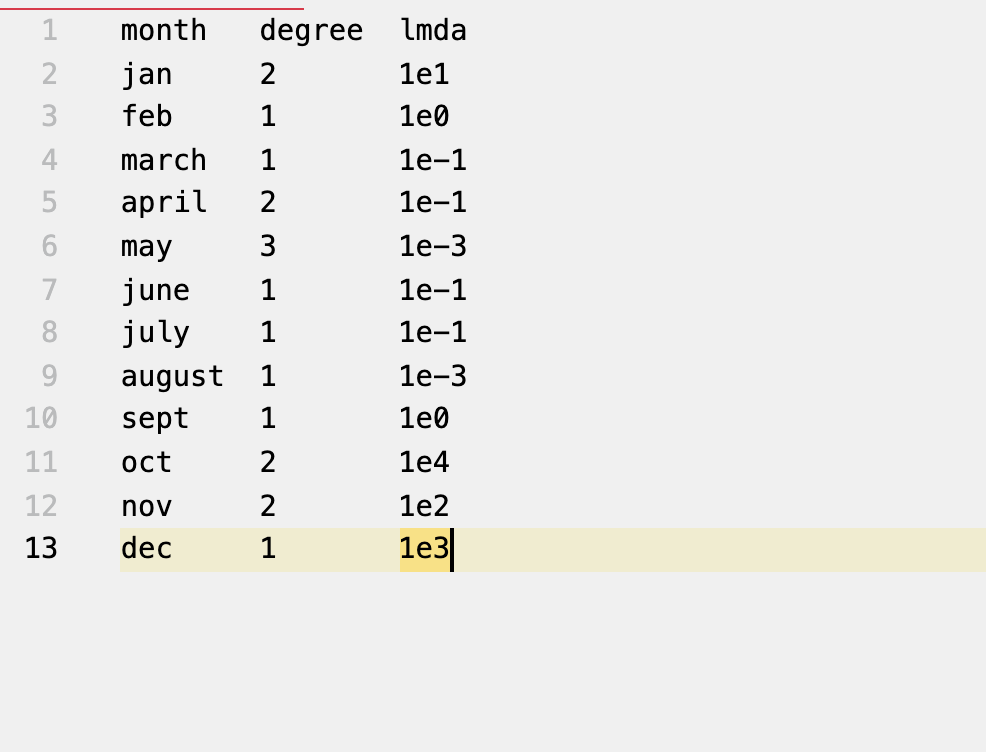
\includegraphics[scale=0.4]{images/37.png}
\end{frame}


\begin{frame}
\begin{huge}
The End
\end{huge}
\end{frame}
\end{document}








